The major part of this thesis was to measure and compare the different synchronization methods and provide a selection basis. To get comparable results, the first step was to choose the hardware and OS for the measurement system. Since the hardware was already given by "Public Devices" with the Raspberry Pi 3 and Linux as the OS, the kernel was the last option to choose.

All measurements were taken under optimal conditions: no CPU load, no RAM load, no storage load, no network load.

\section{Setup}

A detailed installation of the measurement environment is described in Appendix D. The devices connected to a GPS module additionally require the setup described in Appendix C.
The measurements were done with three Raspberry Pis. All of them were connected over Ethernet and a switch. One of them has to transmit a measurement pulse over GPIO 3 to the others' GPIO 2 like described in the "Time vs time" section.

\section{Delays}

A measurement system should provide small latency to get a sharp resolution in time. The popular PREEMPT\_RT patch promises that and was the other option besides the mainline kernel. Both were compiled as described before and exchanged for the different measurements.
Another option to improve latency is to disable the dynamic clock speed of the CPU. This is intended to reduce the power draw in idle situations. But it will increase the latency since important measurement instructions may run on low clock speed in the first place before the kernel reacts to the rising CPU load.

We can divide the delay into different parts. It starts with the internal hardware clock, the OS and the measurement software. Further parts come from the hardware interface, the signal transmission and measurement instrument itself. The aim for this thesis is to minimize the OS delay and provide an overview of interface and transmission delays.

The system delay will tell us which kernel to choose. The accuracy of time synchronization is very much related to the underlying transmission method and provides a first estimation of the error. This error can then be minimized with statistical methods. The delay of the used transmission methods will give an overview.

\subsection{System delay}

The OS delay was measured with the tool cyclictest, which was described before.

\begin{figure}[tb]
	\centering
	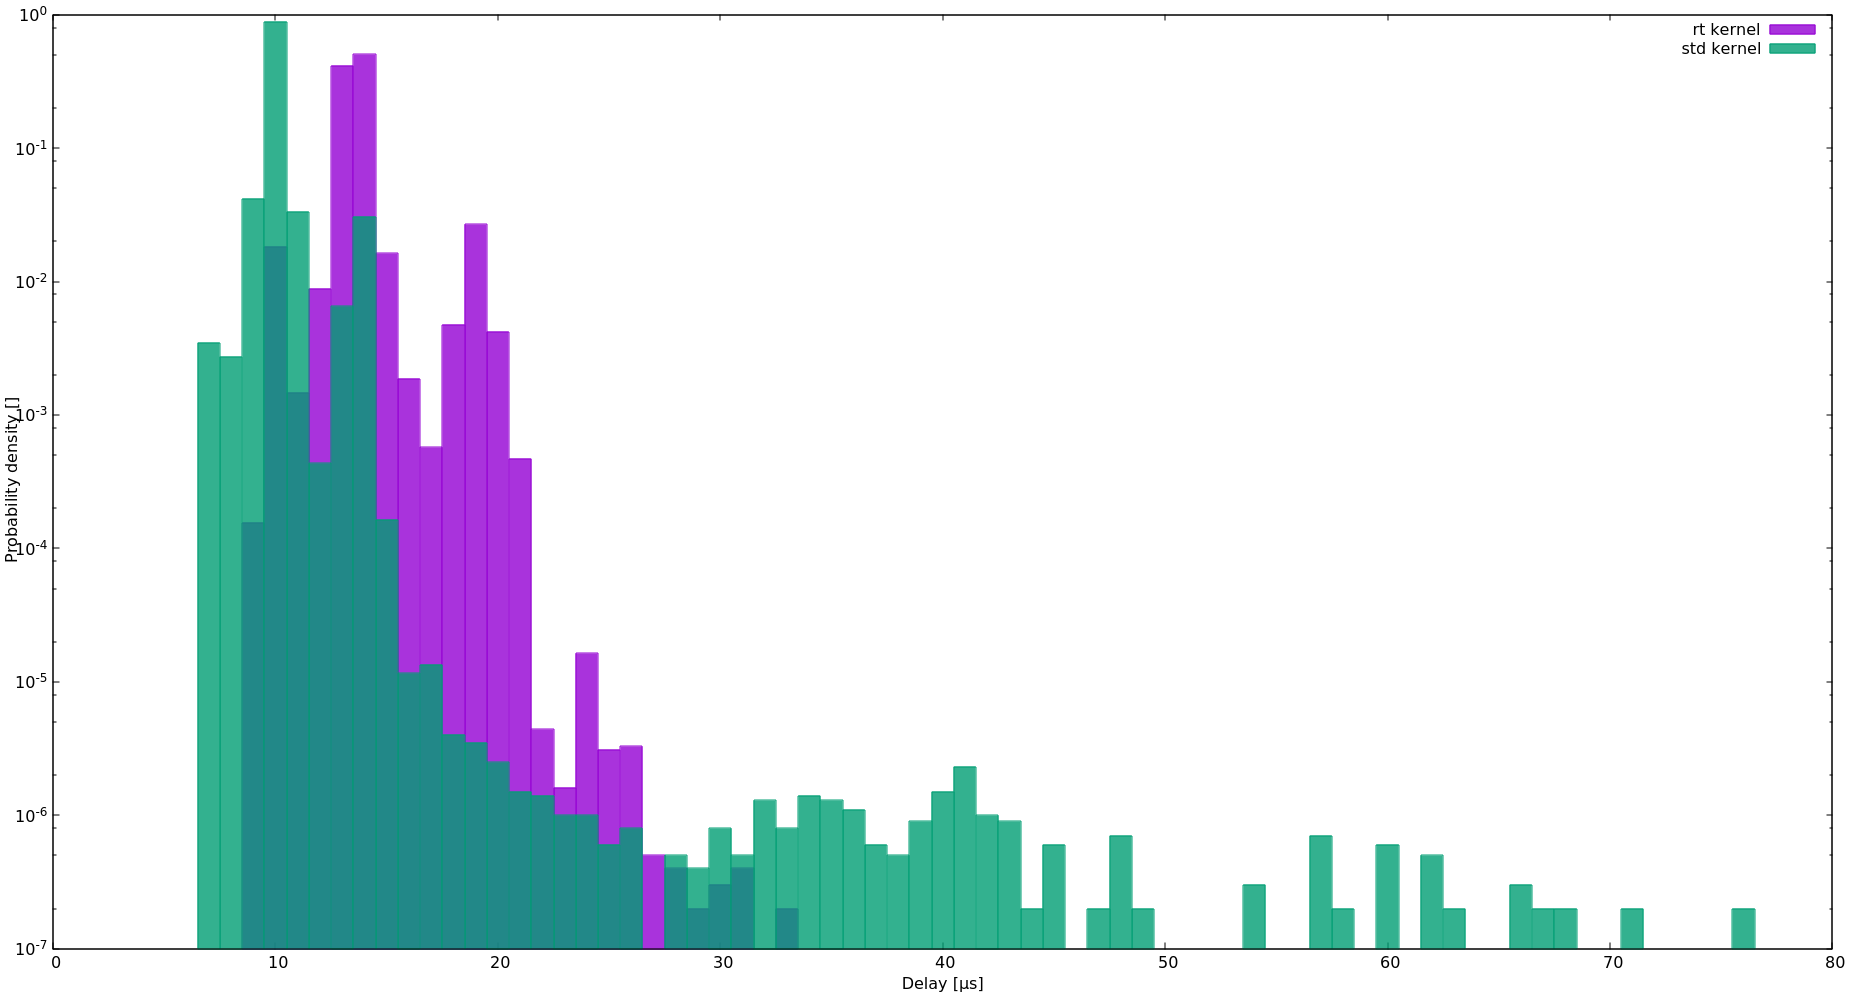
\includegraphics[width=1.0\textwidth]{figures/plot_system.png}
	\caption{System delay}
	\label{fig:plot_system}
\end{figure}

Figure \ref{fig:plot_system} is a plot of the probability density over the delay. Where "rt kernel" stands for the PREEMPT\_RT patched and "std kernel" for the mainline kernel.
As we can see, the PREEMPT\_RT patch gives us a better delimitation but the mainline kernel provides a higher peak with 88\% at 10 µs.

\begin{center}
    \begin{tabular}{ | l | r | r | r | }
    \hline
    \textbf{Target} & \textbf{Delay avg} [µs] & \textbf{Delay min} [µs] & \textbf{Delay max} [µs] \\ \hline
    rt & 13 & 9 & 37 \\ \hline
    std & 10 & 7 & 76 \\ \hline
    \end{tabular}
\end{center}

Issued command:

\begin{lstlisting}[language=bash]
rt-tests/cyclictest -m -t1 -p 99 -n -i 400 -l 10000000 -q -H 400
\end{lstlisting}

\subsection{GPIO delay}

The general-purpose input/output (GPIO) provides a general, easy to use and fast way to generate and process digital signals. Since the Adafruit GPS module has a pulse per second (PPS) signal output, we want to know how accurate this interface is.
To do so, two pins were connected together, one used as an output and the other as an input. Then the time difference between generating and receiving an impulse it is taken. This was repeated for a period of time to get a smooth delay distribution.

\begin{figure}[tb]
	\centering
	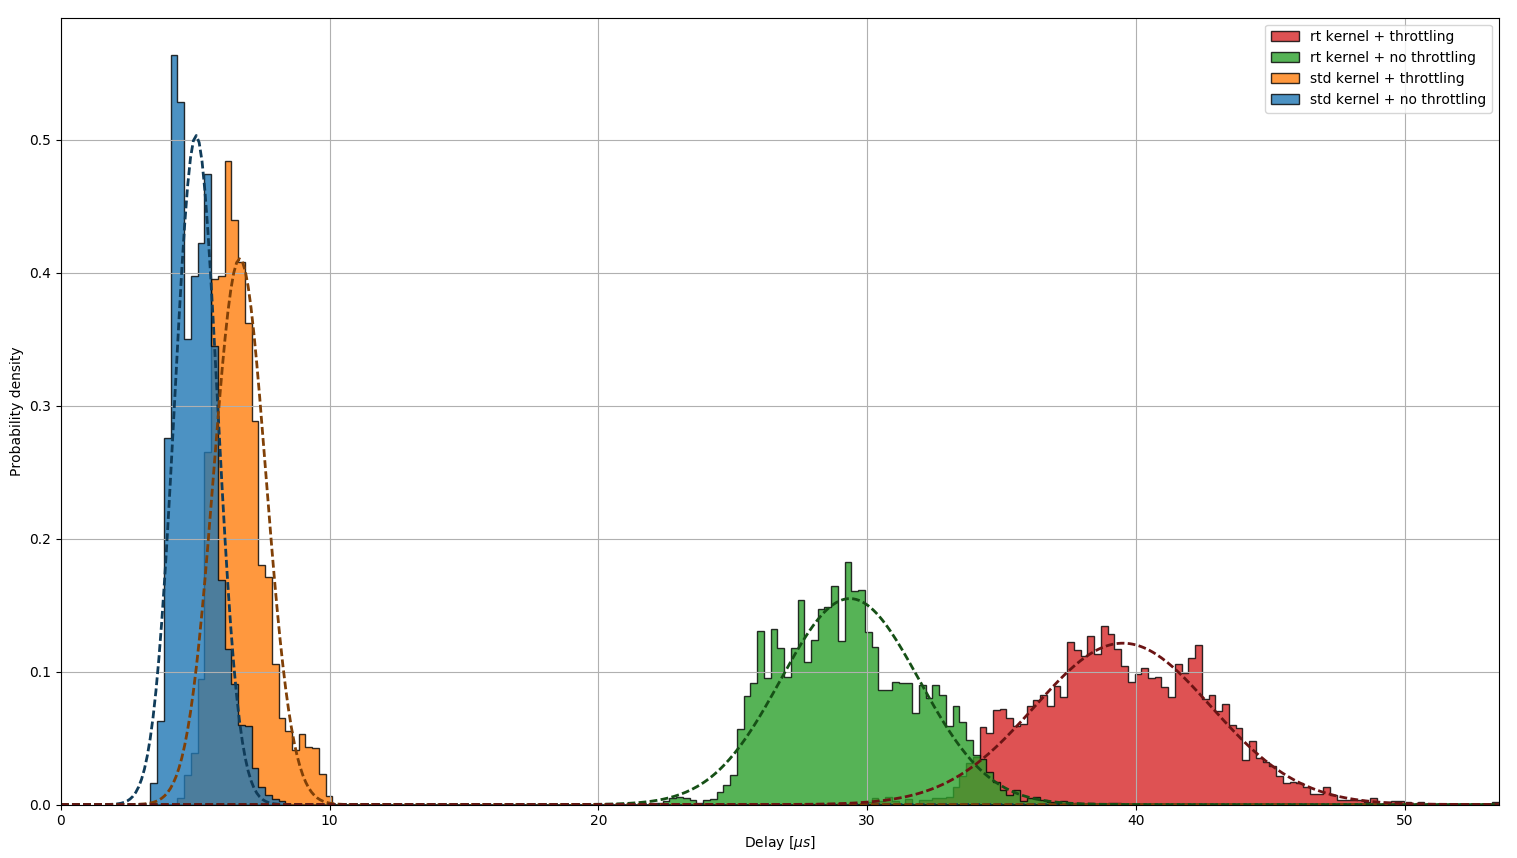
\includegraphics[width=1.0\textwidth]{figures/plot_gpio.png}
	\caption{GPIO delay}
	\label{fig:plot_gpio}
\end{figure}

The measured distributions are shown in Figure \ref{fig:plot_gpio}. Where "rt kernel" stands for the PREEMPT\_RT patch and "std kernel" for the standard mainline kernel. In addition, the CPU was configured to stay with a single frequency designated with "no throttling" and the default configuration with "throttling".
As we can see, configuring the Raspberry Pi to not adopt the CPU's frequency has a noticeable impact on the delay. The latency with the PREEMPT\_RT patch is not only about 6 times higher, but also more spread out. A wider distribution will also cause a higher error for a time synchronization method that relies on GPIO like GPS.

The enveloping gaussians are parameterized as the following:

\begin{center}
    \begin{tabular}{ | l | r | }
    \hline
    \textbf{Target} & \textbf{Delay} [µs] \\ \hline
    std kernel + no throttling & 5.0\pm 0.8 \\ \hline
    std kernel + throttling & 6.7\pm 1.0 \\ \hline
    rt kernel + no throttling & 29.4\pm 2.5 \\ \hline
    rt kernel + throttling & 39.5\pm 3.3 \\ \hline
    \end{tabular}
\end{center}

The static CPU frequency was configured by adding the following lines to /boot/config.txt:
\begin{lstlisting}[language=bash]
# static frequency
force_turbo=1
arm_freq=800
arm_freq_min=800
\end{lstlisting}

Issued commands:

\begin{lstlisting}[language=bash]
time-tools/measure-server -i 0.5 &
time-tools/measure-client 127.0.0.1 &
\end{lstlisting}

\subsection{Network delay}

The network delay is very important for NTP and PTP. The delay distribution gives a first estimation of the synchronization error. With the assumption that the delay is the same in both directions and it doesn't vary too much, the error can be reduced by statistical methods like described in the NTP and PTP chapter.

\begin{figure}[tb]
	\centering
	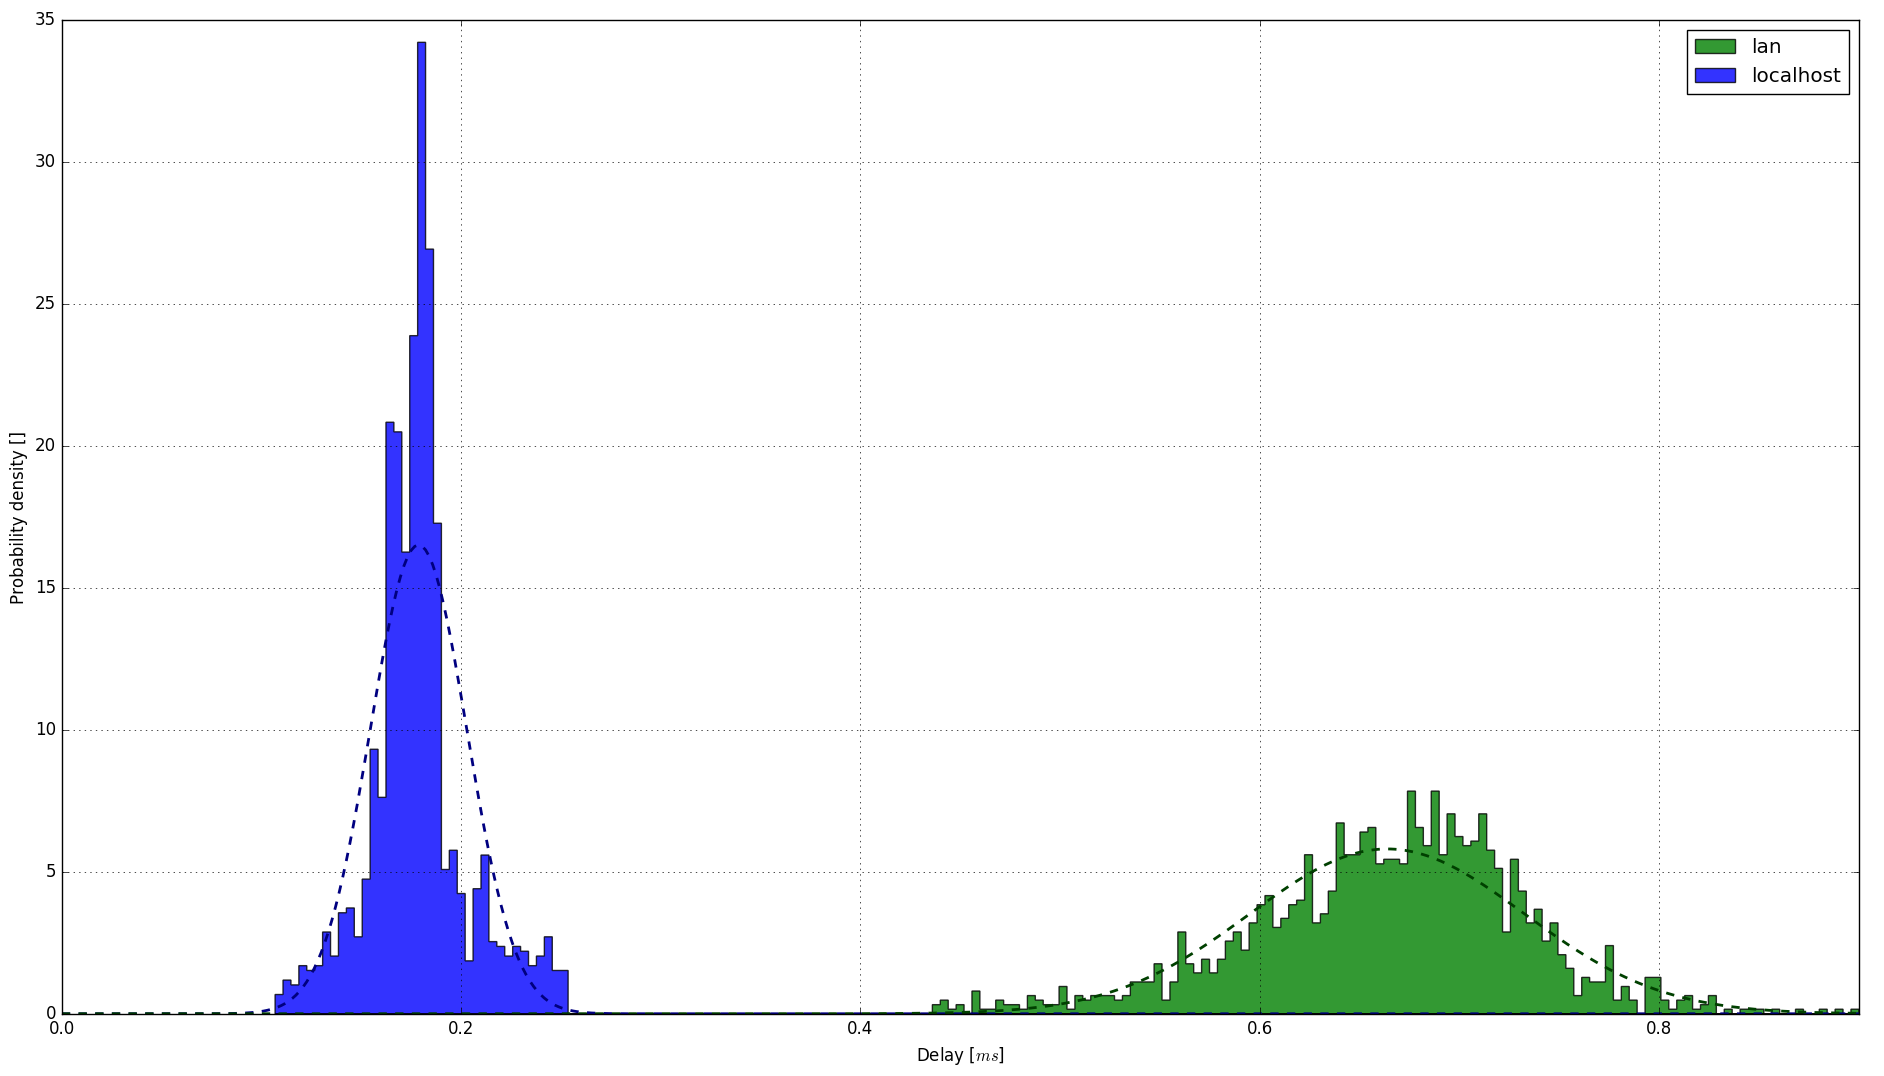
\includegraphics[width=1.0\textwidth]{figures/plot_network.png}
	\caption{Network delay}
	\label{fig:plot_network}
\end{figure}

The measured distributions are shown in Figure \ref{fig:plot_network}. The localhost measured to get an idea of what delay is caused by the OS itself. For a LAN attached device we get a similar distribution like "lan". It fits the gaussian distribution very well.

The enveloping gaussians are parameterized as the following:

\begin{center}
    \begin{tabular}{ | l | r | }
    \hline
    \textbf{Target} & \textbf{Delay} [ms] \\ \hline
    localhost & 179\pm 24 \\ \hline
    lan & 664\pm 69 \\ \hline
    internet & 25634\pm 213 \\ \hline
    \end{tabular}
\end{center}

Issued command:

\begin{lstlisting}[language=bash]
delay-icmp <host>
\end{lstlisting}

\subsection{NMEA delay}

Since the GPS module has two different transmission methods to emit a second, a calibration is required. While the PPS line gives us a single digital pulse when a UTC second has started, the serial connection tells us which second it was. The delay between those two can be measured and passed to the NTP daemon.

The delay was measured with: (435\pm 89) ms

Issued command:

\begin{lstlisting}[language=bash]
delay-nmea -s ~/time-experiments.c/nmea_pulse /dev/ttyS0 ~/time-experiments.c/pps_pulse /dev/pps0
\end{lstlisting}

\section{Time deviation}

The following measurements were taken to see the moving time offset of connected Raspberry Pis to a chosen norm. With the help of that we can visualize the process of time synchronization with a resolution of a few µs.

The three Raspberry Pis were called \textit{rpi1}, \textit{rpi2} and \textit{rpi3}. \textit{rpi1} was chosen to be the server and therefore the norm to compare to. The two GPS modules were connected to \textit{rpi1} and \textit{rpi2}. In order to measure the time accurately the server is connected to all his clients with per GPIO and Ethernet. A digital pulse is emitted by \textit{rpi1} to the others. The clients take a timestamp and send it back to the server over UDP.

Before the measurement is started, the client clocks are synchronized to be within 1-2 seconds and the kernel clock parameters are screwed.

This is a summary of the required measurement commands:

\begin{lstlisting}[language=bash]
# server commands
time-tools/measure-server -i 0.5
time-config time-tools/tconfig/config-...

# client commands
time-tools/tsync rpi1 1
time-tools/screwclock
time-tools/measure-client rpi1
time-config time-tools/tconfig/config-...
\end{lstlisting}

At first we will see how an unsynchronized clocks behaves. Followed by using NTP, PTP and GPS. After that we will compare them in the next chapter. All following measurements were taken with the mainline kernel and constant CPU clock rate.

\subsection{Nonlinear deviation}

This measurement was taken to see what happens to a clock without a continuous synchronization. It is summarized in Figure \ref{fig:plot_nonlinear}.

\begin{figure}[tb]
	\centering
	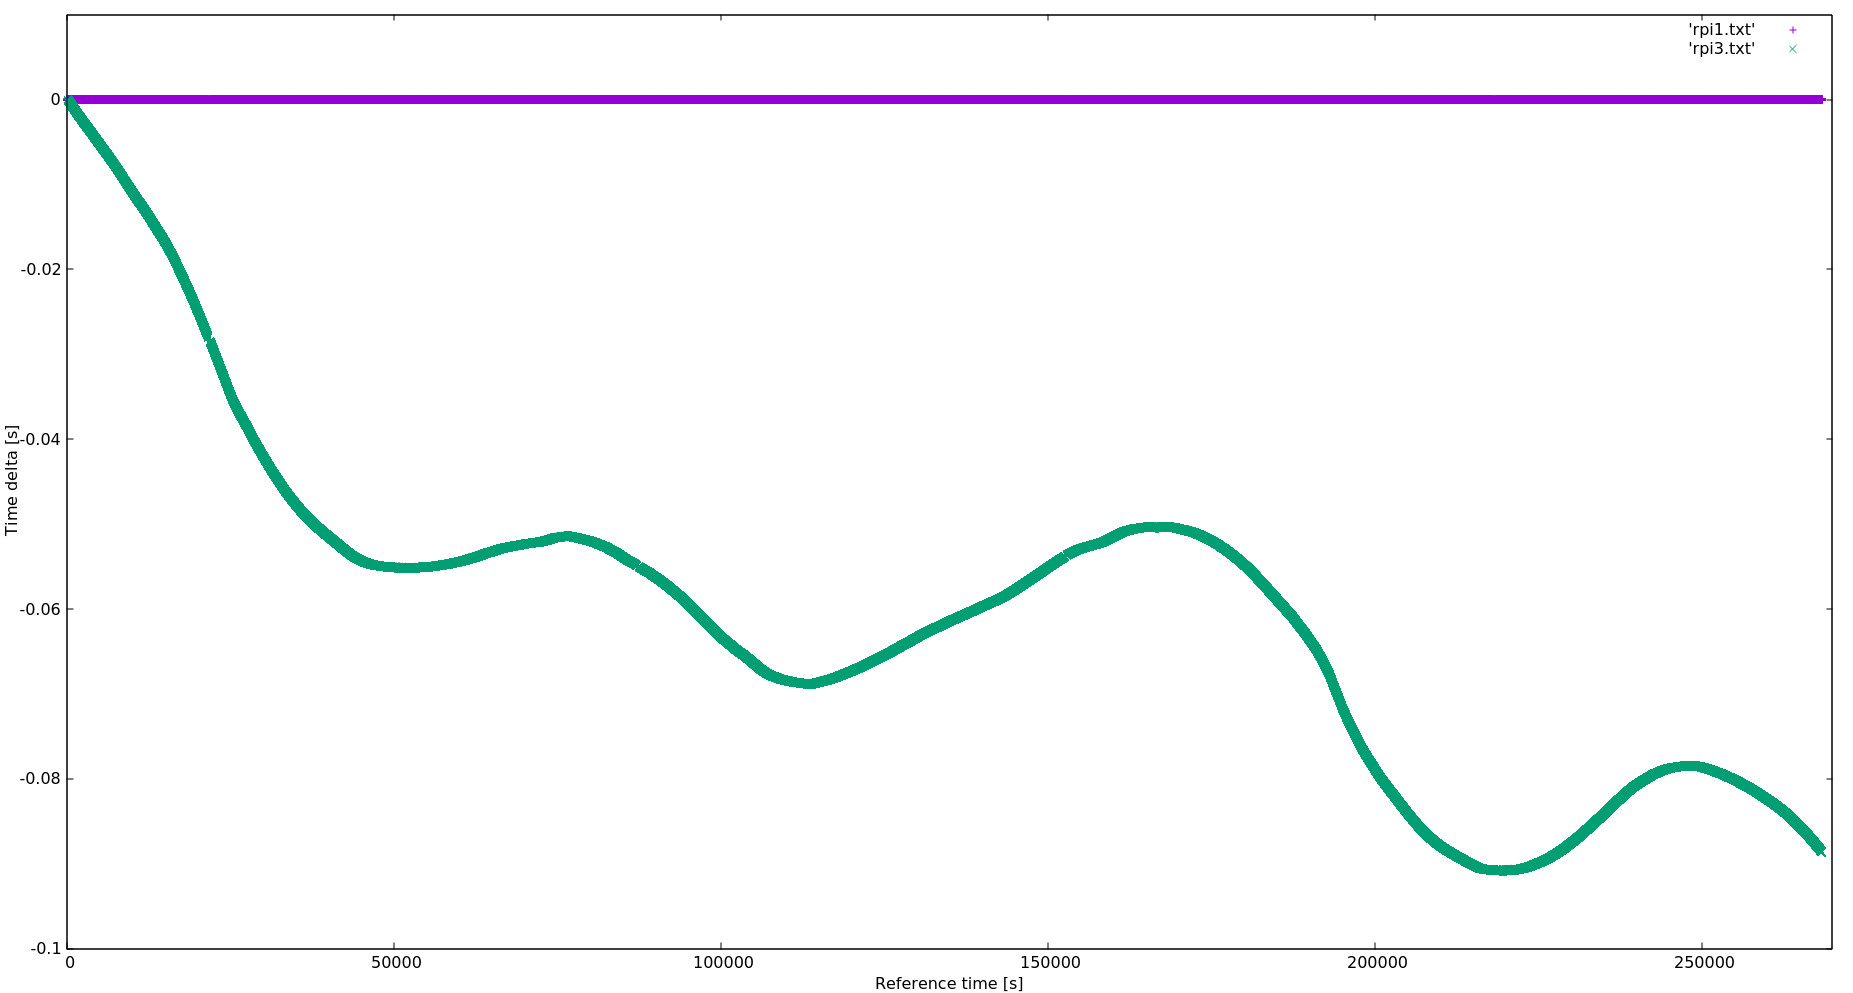
\includegraphics[width=1.0\textwidth]{figures/plot_nonlinear.png}
	\caption{Nonlinear deviation}
	\label{fig:plot_nonlinear}
\end{figure}

The reference clock \textit{rpi1} was synchronized by GPS while the clock of \textit{rpi3} was on its own. With about 3 days of measuring and the accompanying temperature fluctuations we can see that clock synchronization needs both: phase and frequency adjustment.
The measurement was started at 12:00 AM. We can see that the clock frequency is connected to the changing ambient temperature caused by the day cycle and weather.

\subsection{NTP}

The following measurement was taken with \textit{rpi1} as reference clock, \textit{rpi2} and \textit{rpi3} as synchronization targets.

\begin{figure}[tb]
	\centering
	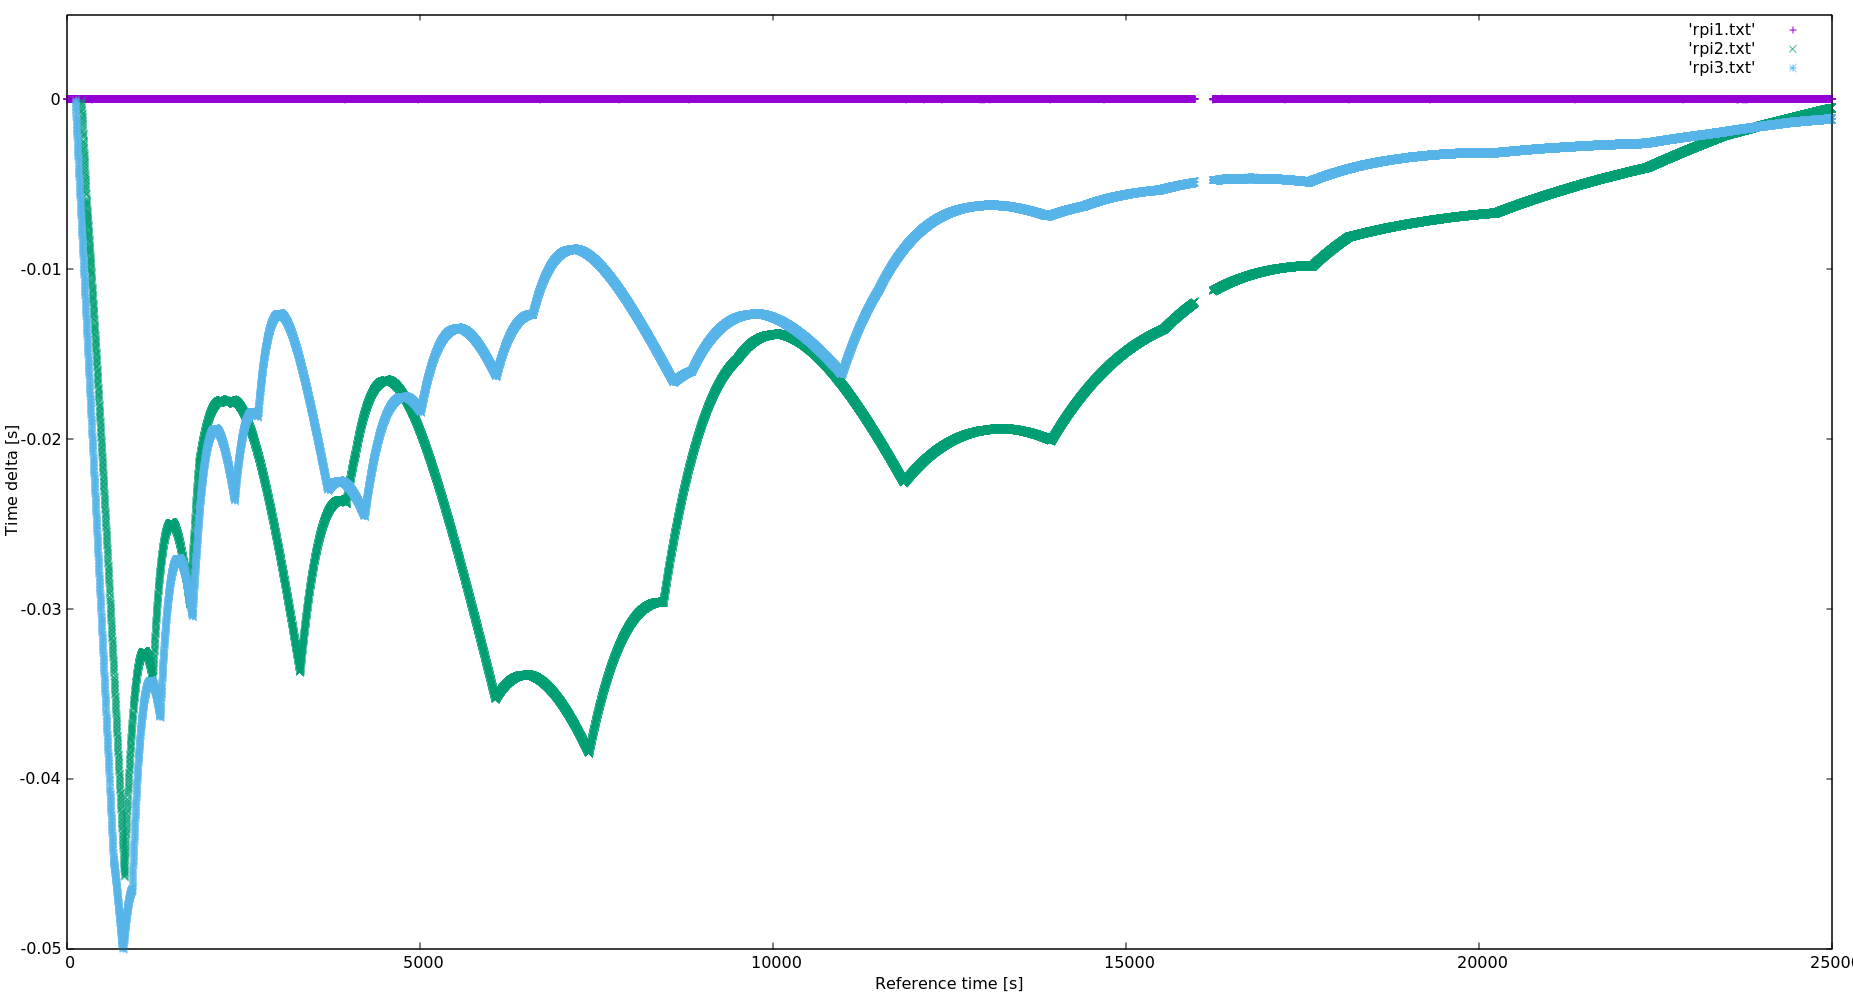
\includegraphics[width=1.0\textwidth]{figures/plot_ntp1.png}
	\caption{NTP synchronization}
	\label{fig:plot_ntp1}
\end{figure}

We can see the synchronization process in Figure \ref{fig:plot_ntp1}. With the initiation of the NTP daemon the target clock's phase is adjusted to about 0.1 ms relative to the reference clock. Then the frequency adjustment begins. In this case the target's clock frequency is very badly conditioned in comparison to the reference. NTP took about 14 h to fix this issue. Figure \ref{fig:plot_ntp2} shows the continuous time oscillation after the synchronization is done. This leads to an accuracy of about 0.2 ms.

\begin{figure}[tb]
	\centering
	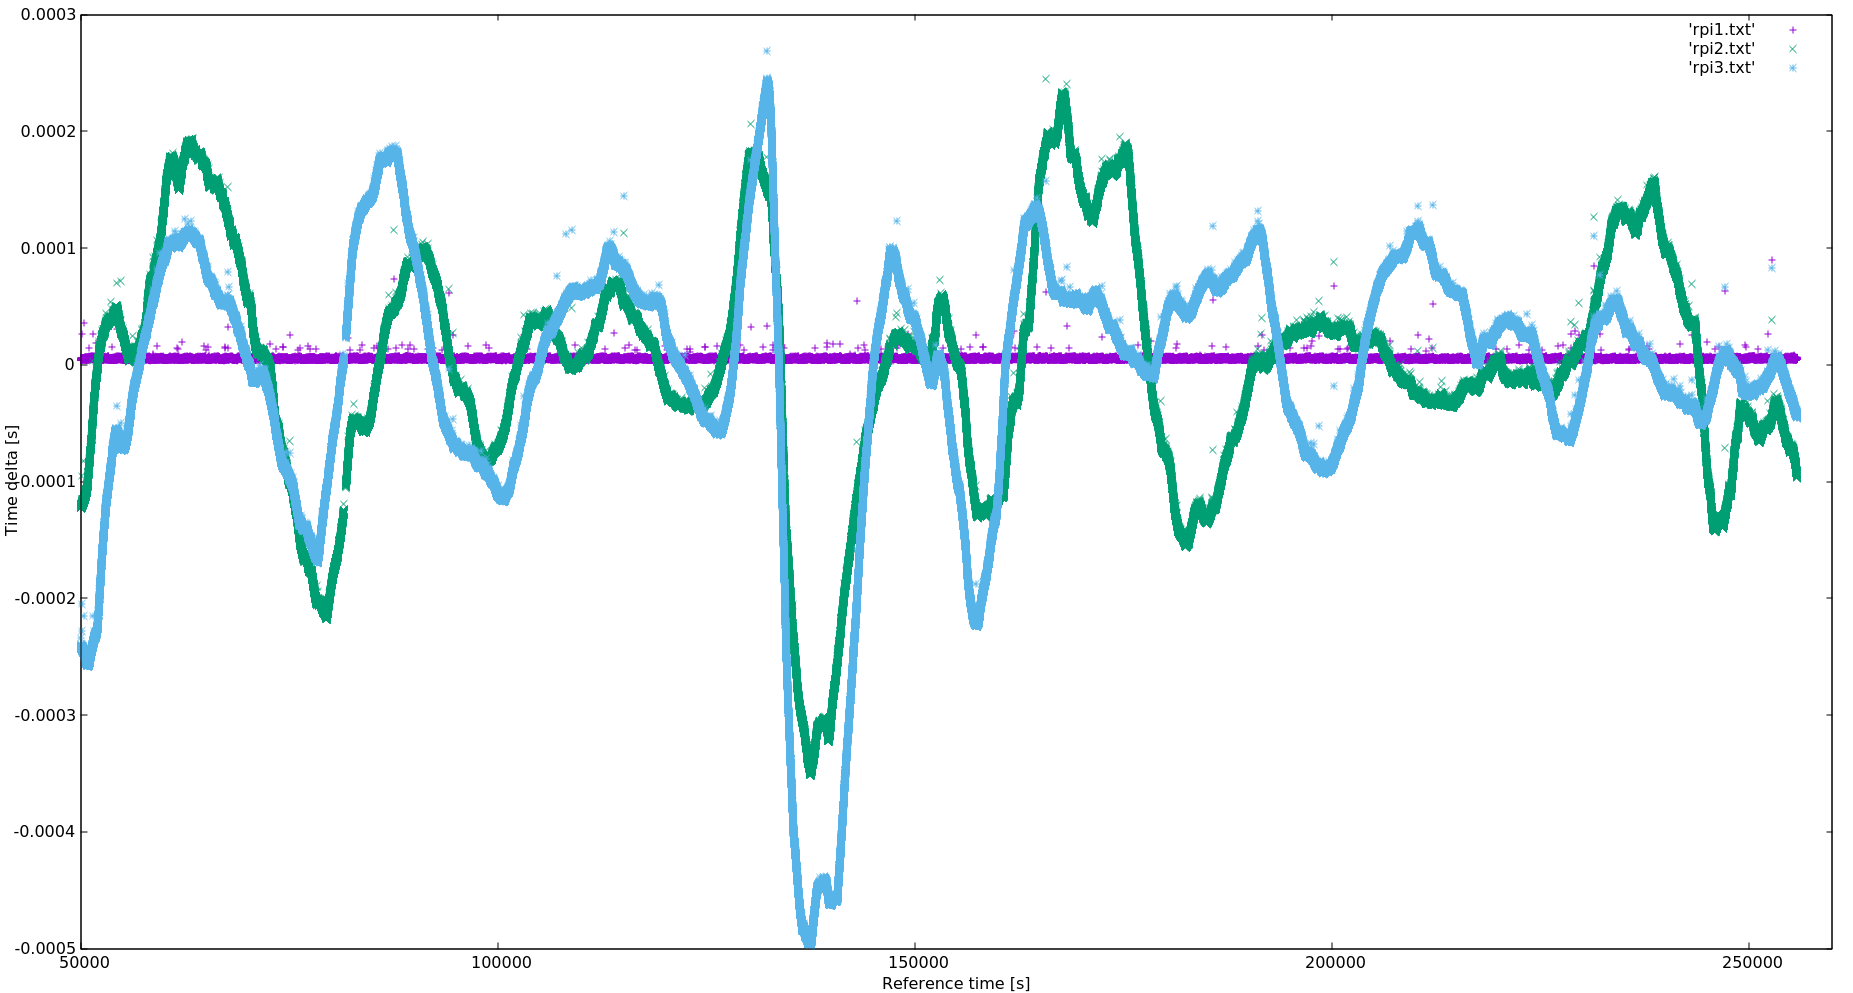
\includegraphics[width=1.0\textwidth]{figures/plot_ntp2.png}
	\caption{NTP accuracy}
	\label{fig:plot_ntp2}
\end{figure}

\subsection{PTP}

The topological setup is the same as before: \textit{rpi1} as reference clock, \textit{rpi2} and \textit{rpi3} as synchronization targets.

\begin{figure}[tb]
	\centering
	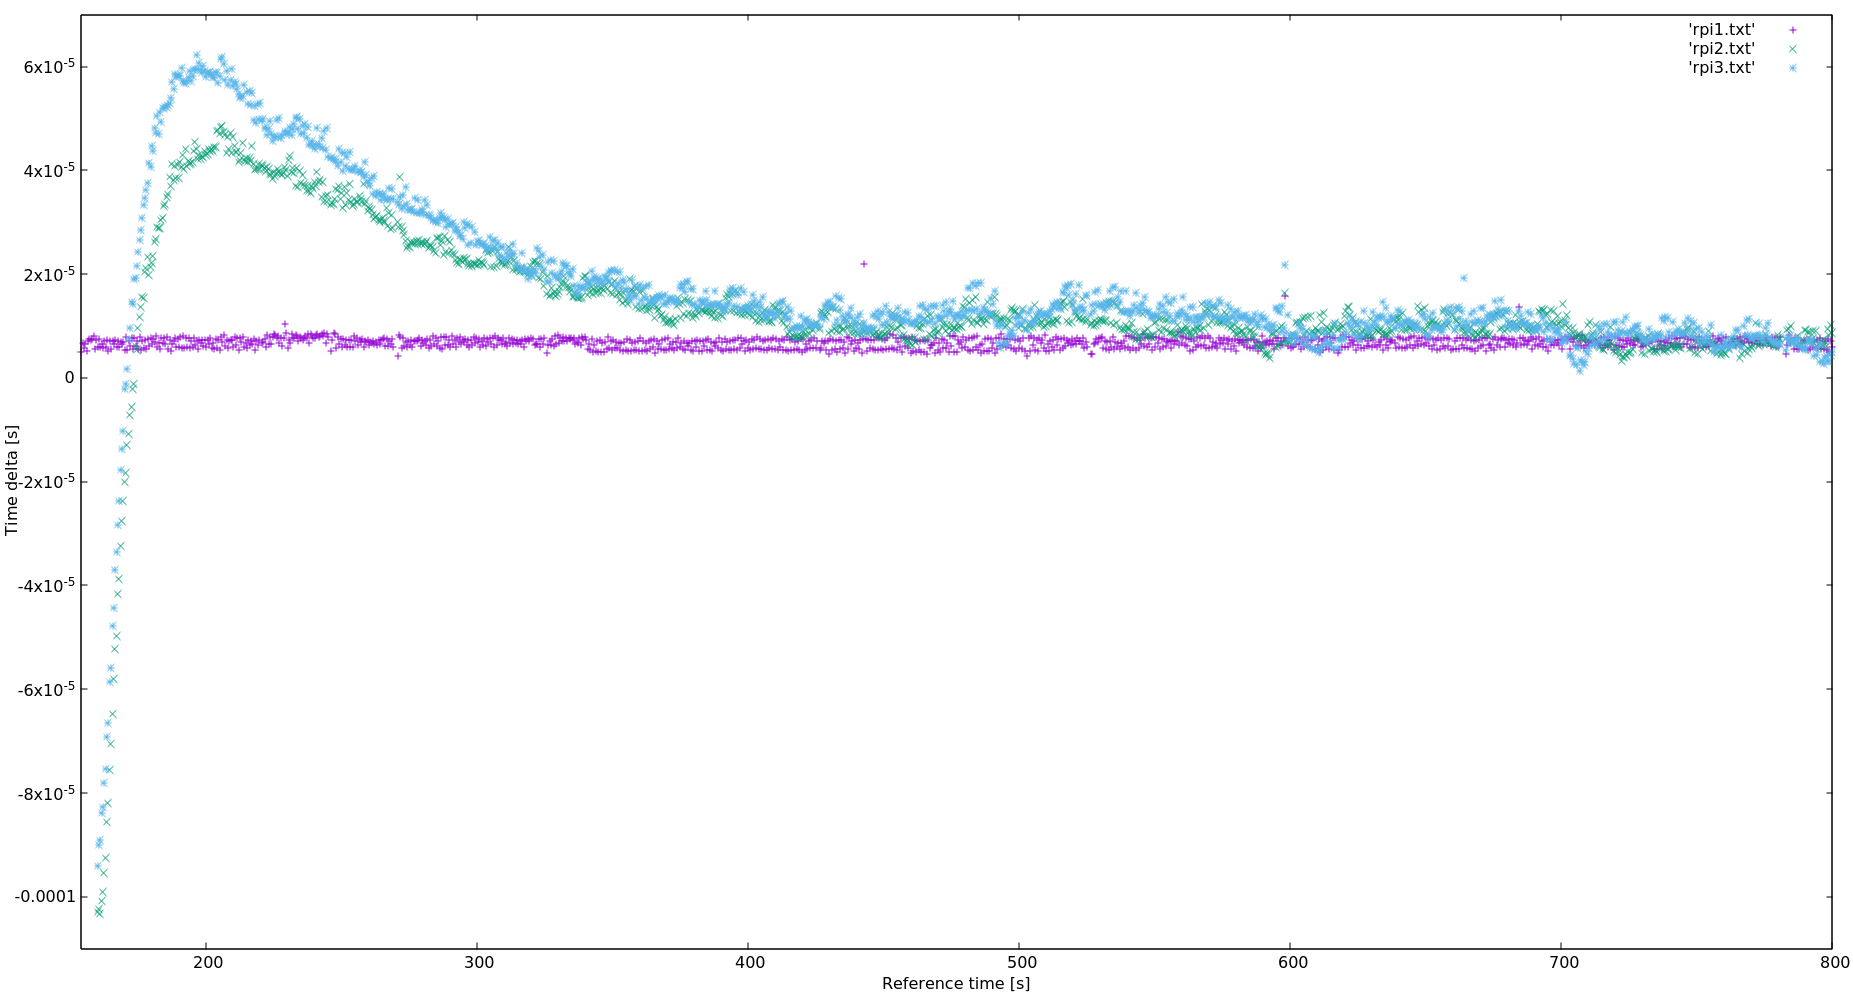
\includegraphics[width=1.0\textwidth]{figures/plot_ptp1.png}
	\caption{PTP synchronization}
	\label{fig:plot_ptp1}
\end{figure}

With the initiation of the PTP daemon the target's clock phase is adjusted to about 0.1 ms relative to the reference clock like shown in Figure \ref{fig:plot_ptp1}. The frequency adjustment takes over and completes in about 6 minutes. The accuracy gets very close to the measurement error with about 10 µs as we can see in Figure \ref{fig:plot_ptp2}.

\begin{figure}[tb]
	\centering
	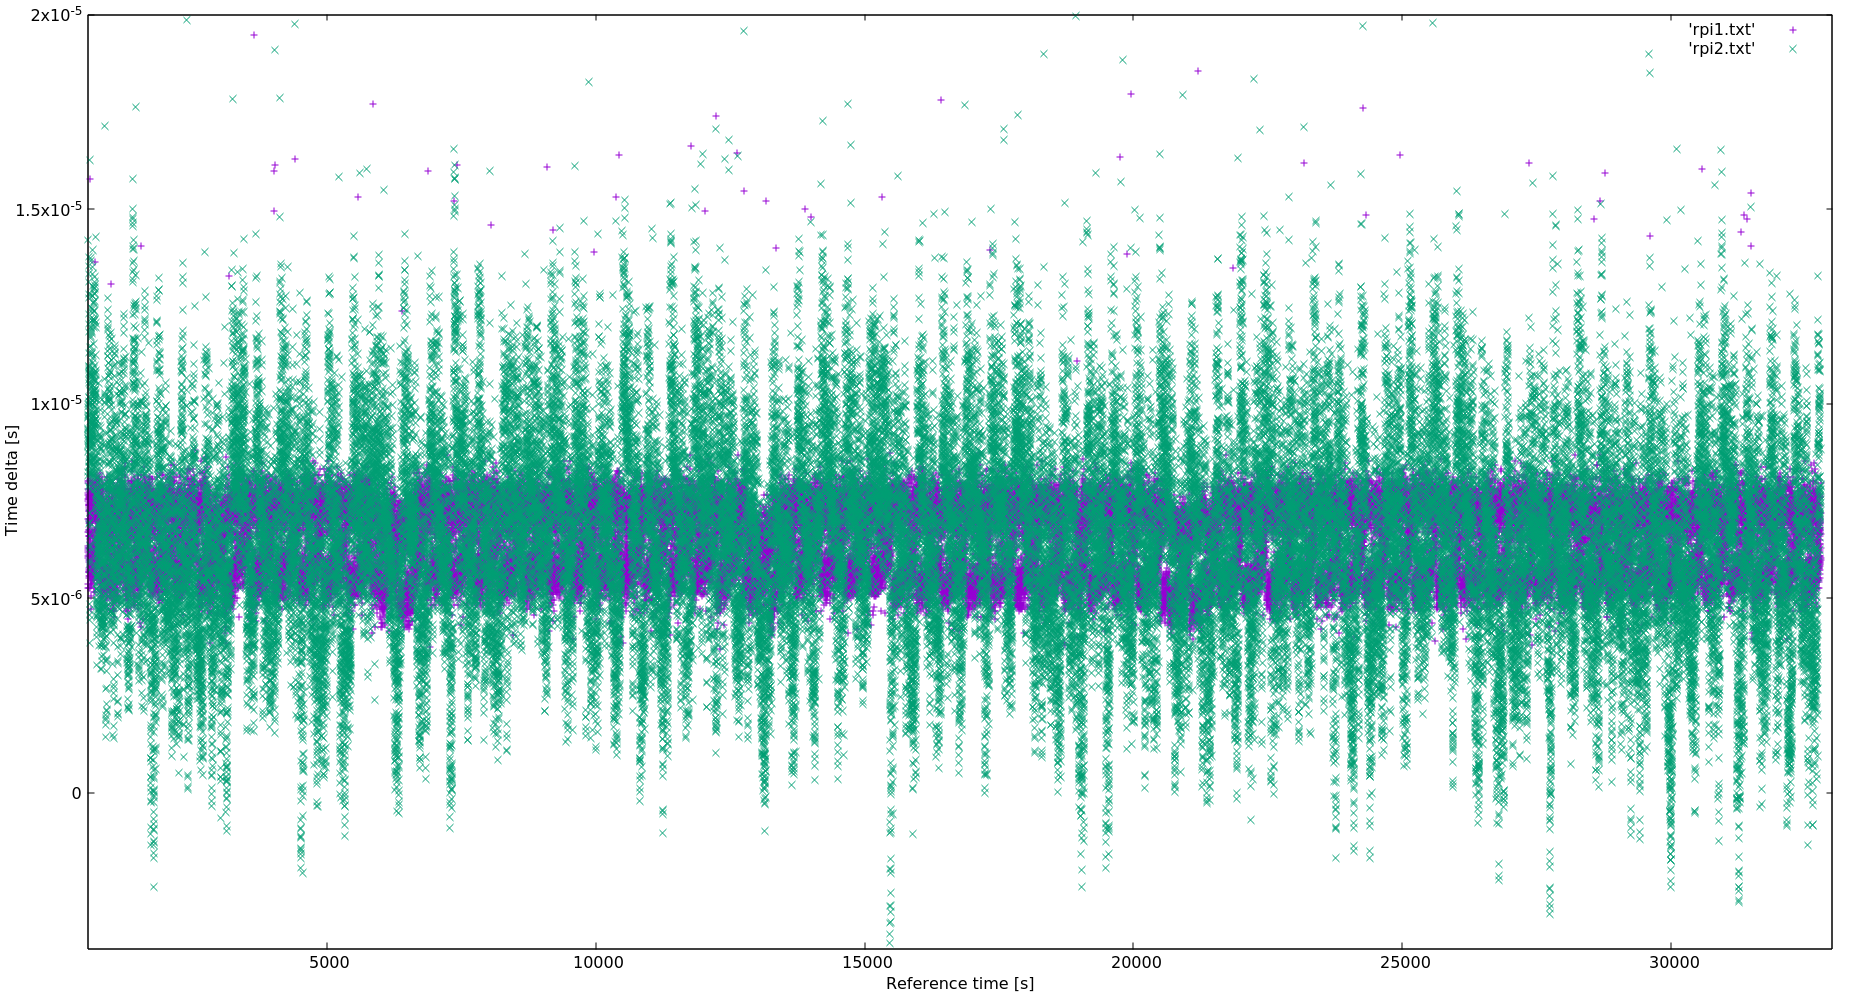
\includegraphics[width=1.0\textwidth]{figures/plot_ptp2.png}
	\caption{PTP accuracy}
	\label{fig:plot_ptp2}
\end{figure}

\subsection{GPS}

To get an estimate of the error, two GPS modules are required in order to compare them. \textit{rpi1} was started and synchronized long before \textit{rpi2}. With this way we have a stable reference to compare to and follow the initial time synchronization of \textit{rpi2}.

\begin{figure}[tb]
	\centering
	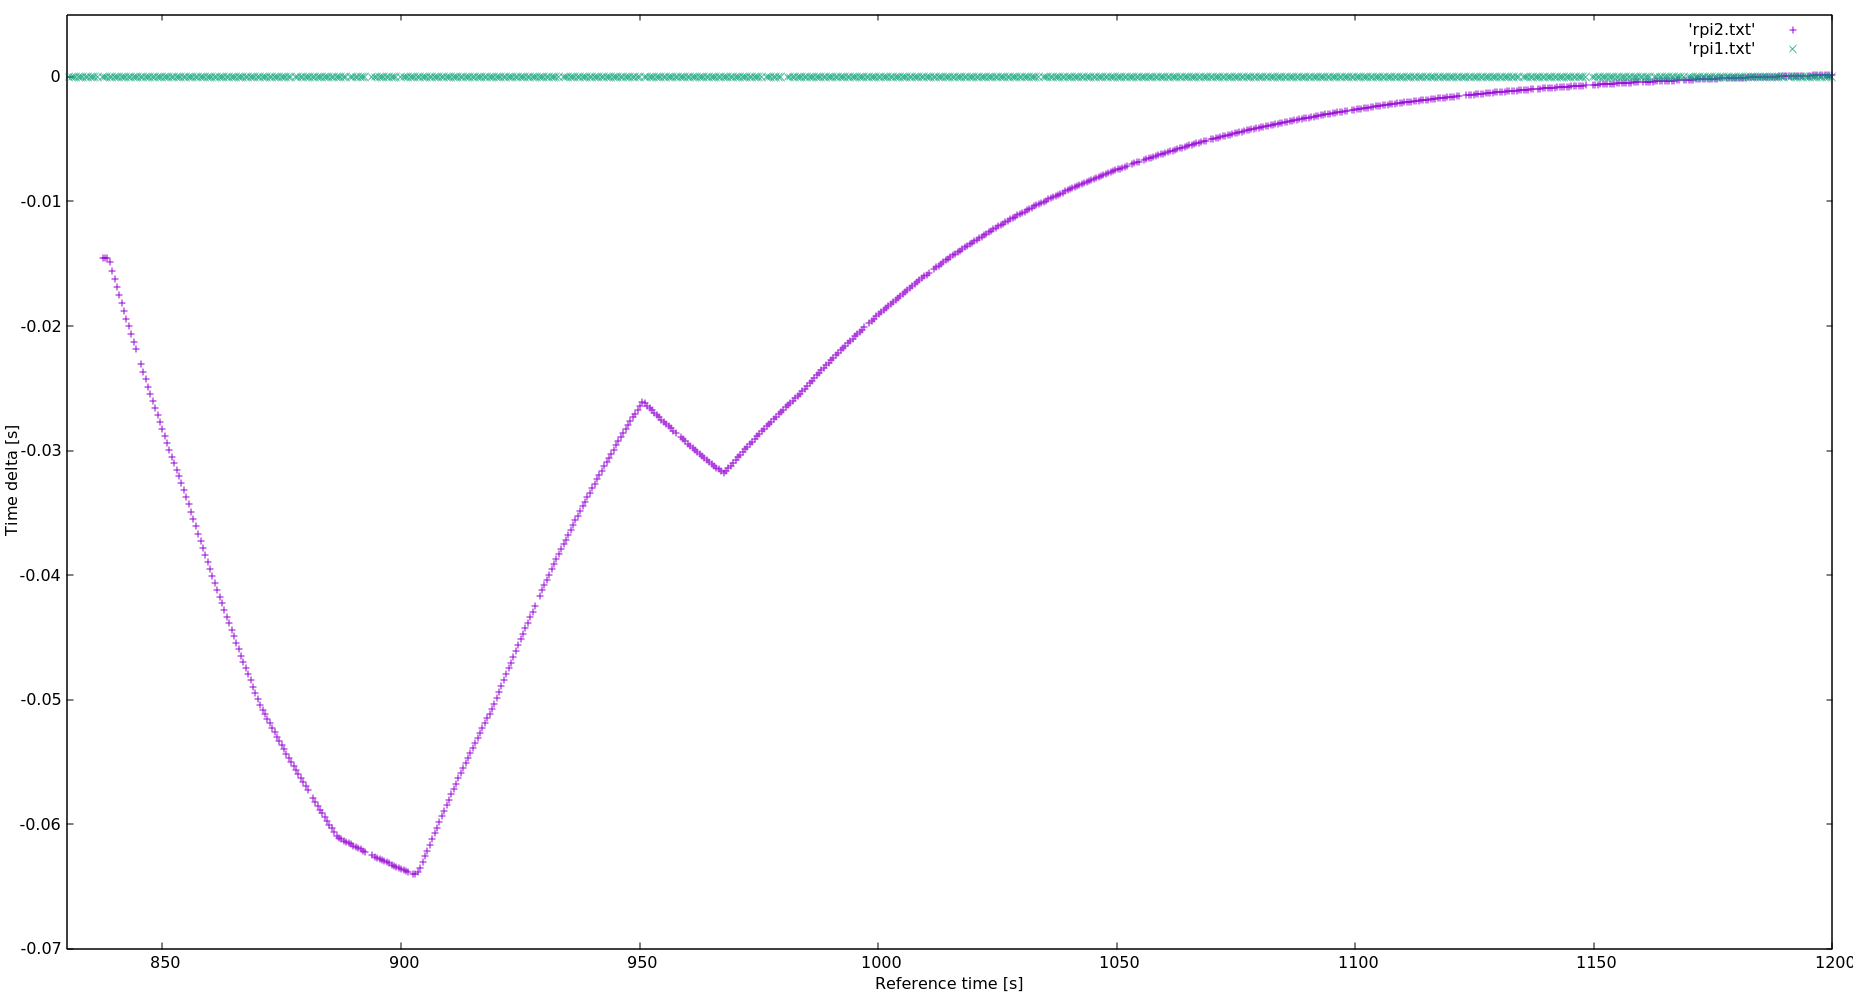
\includegraphics[width=1.0\textwidth]{figures/plot_gps1.png}
	\caption{GPS synchronization}
	\label{fig:plot_gps1}
\end{figure}

\begin{figure}[tb]
	\centering
	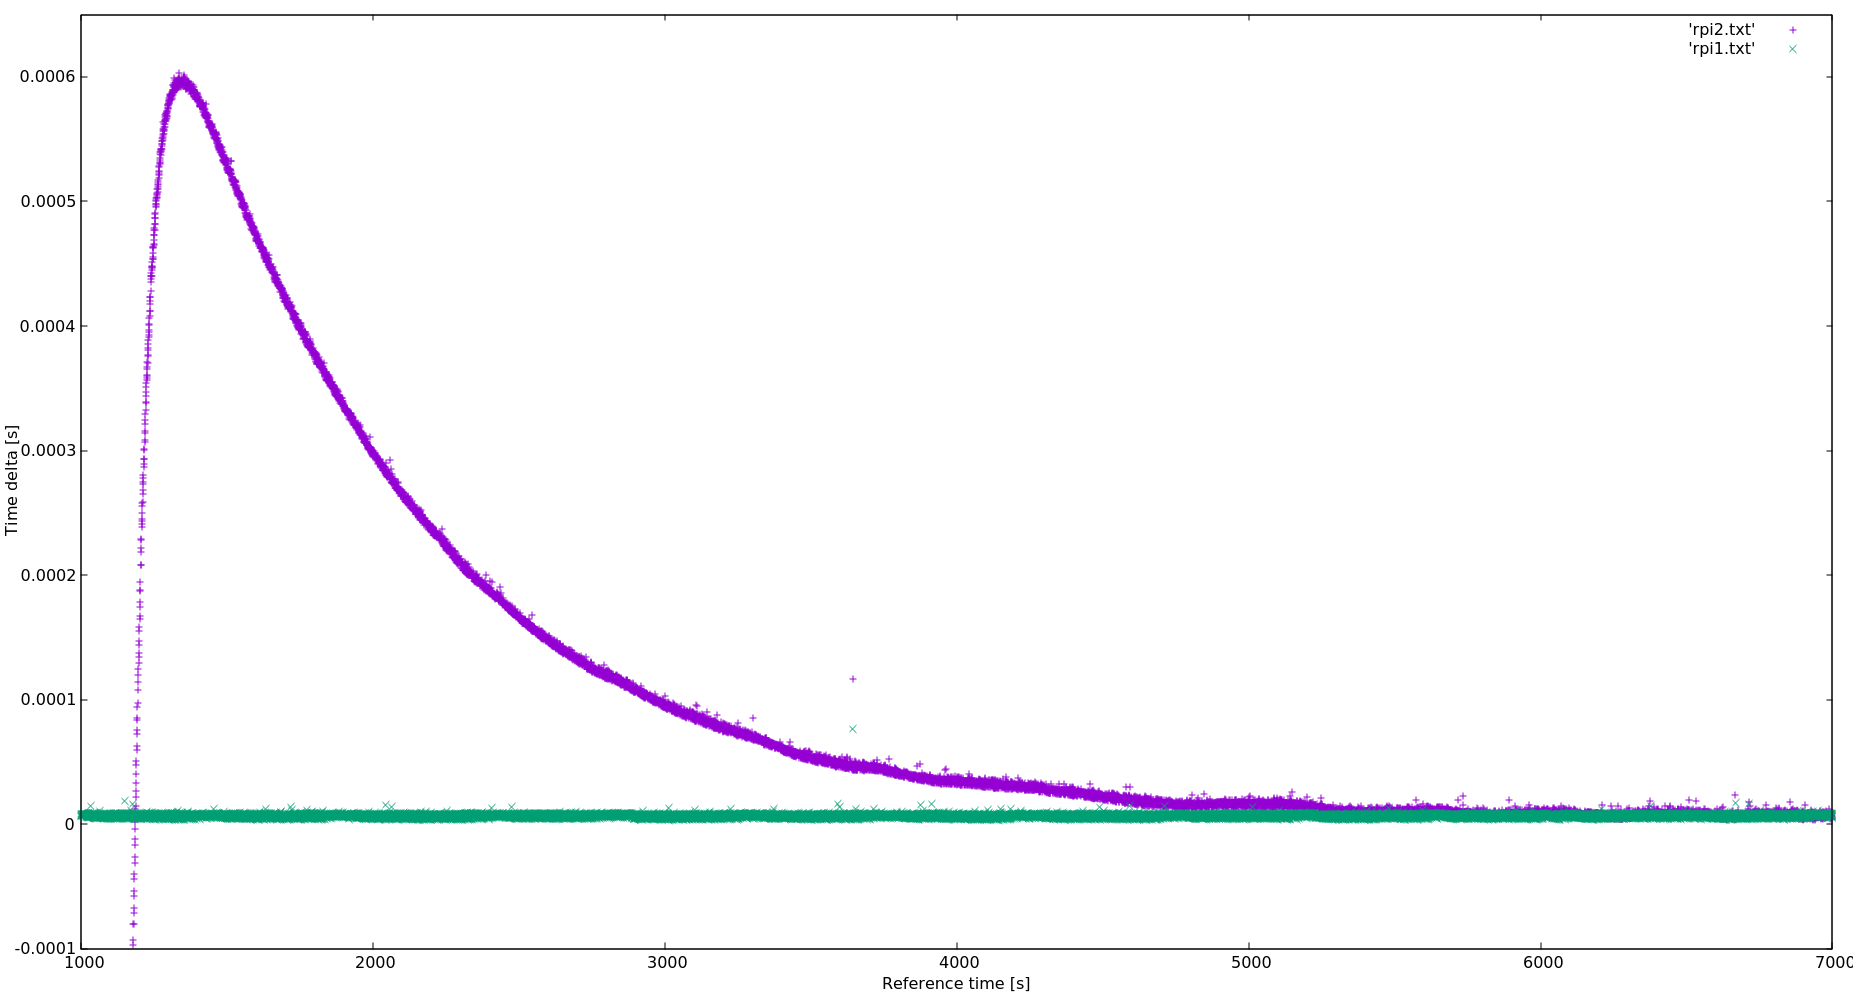
\includegraphics[width=1.0\textwidth]{figures/plot_gps2.png}
	\caption{GPS synchronization close-up}
	\label{fig:plot_gps2}
\end{figure}

The initiation of the NTP daemon with GPS configuration adjusts the phase to about 10 ms relative to the reference clock like shown in Figure \ref{fig:plot_gps1}. The high error comes from the serial connection. NTP starts using the serial interface first and heads over to PPS after analyzing the signal. After about 2 minutes the PPS signal gets accepted, followed by a slow converging curve towards reference within about 90 minutes shown in Figure \ref{fig:plot_gps2}.

\begin{figure}[tb]
	\centering
	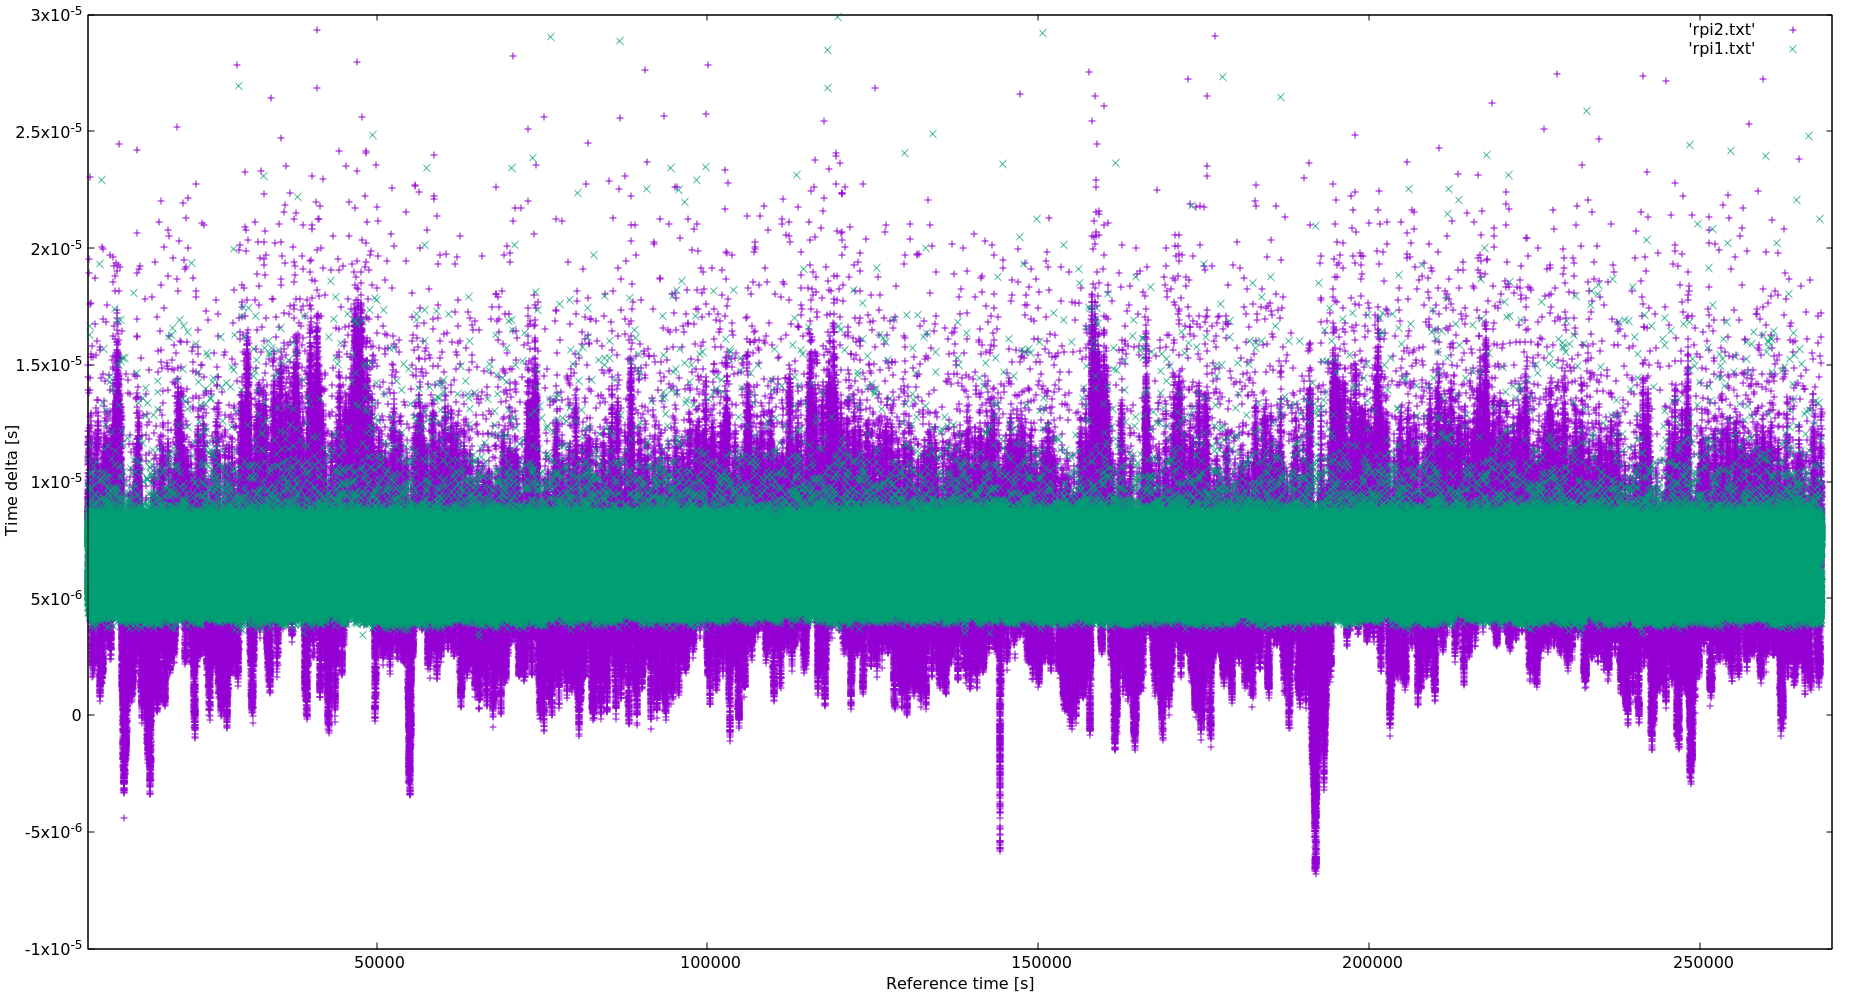
\includegraphics[width=1.0\textwidth]{figures/plot_gps3.png}
	\caption{GPS accuracy}
	\label{fig:plot_gps3}
\end{figure}

In the end we reach an accuracy close to the measurement error of about 10 µs illustrated by Figure \ref{fig:plot_gps3}.

